\documentclass [12pt] {beamer}
%\usepackage{beamerthemeDarmstadt}
% \usepackage{beamerthemeCambridgeUS}
\usepackage{beamerthemeWarsaw}
%  \useoutertheme{shadow}
\usecolortheme{crane}
%  \useoutertheme{miniframes}
% \usecolortheme{wolverine}
\usepackage{graphicx}
\setbeamercovered{transparent}

\title{Cloud Computing \& Networking Of Information}
\author{Kiran.V.}
\date{\today}
% \department{CSE}
\institute {Guided By : Mr.Aneesh M Haneef, \\Asst: Professor \\CSE Department M.E.S CE}

\begin{document}
\frame{\titlepage}

\section{Agenda}
\tableofcontents

\section{Cloud Computing}
\begin{frame}
\begin{center}
 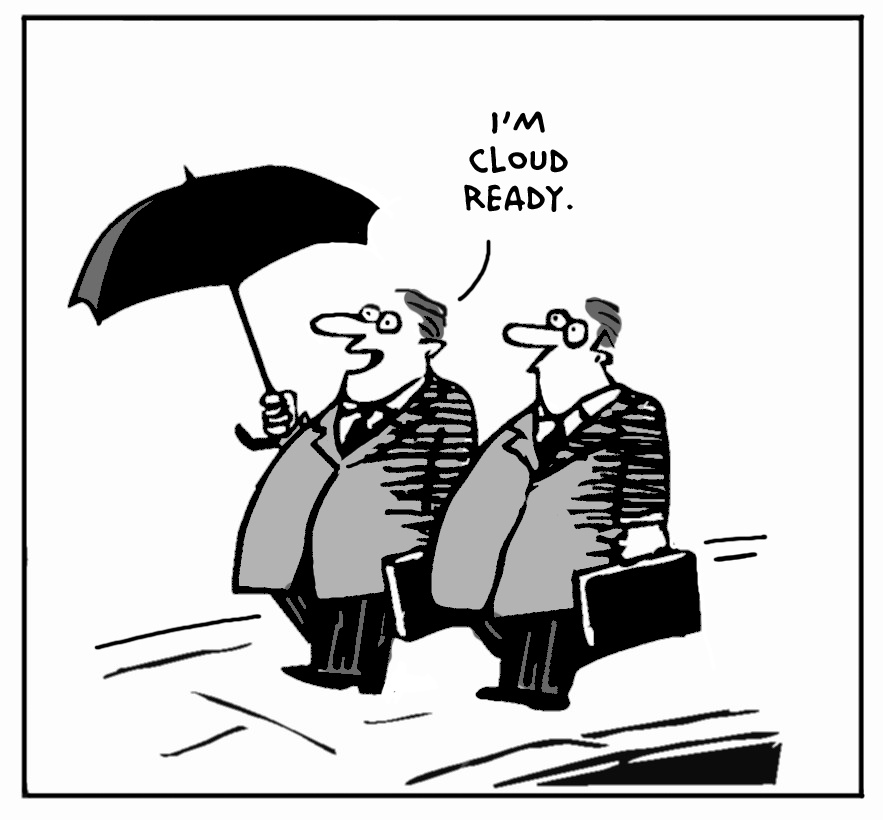
\includegraphics[1.25]{CC1.jpg}
\end{center}
\end{frame}

\begin{frame}
 \begin{center}
  \emph{\textbf{C}ommon, \textbf{L}ocation-independent, \textbf{O}nline \textbf{U}tility that is available on \textbf{D}emand}
 \end{center}

\end{frame}



\begin{frame}
\frametitle{Cloud Computing}
\begin{itemize}
 \item <1-> Delivery as a service rather than a product.
 \item <2-> Marketing term for technologies providing computation, software, data access and storage services.
 \item <3-> Applications Delivered via Internet.
 \item <4-> Bussiness software and data stored in servers.
\end{itemize}
\end{frame}

\subsection{Layers of Cloud Computing}
\begin{frame}
\frametitle{Layers of Cloud Computing}
\begin{center}
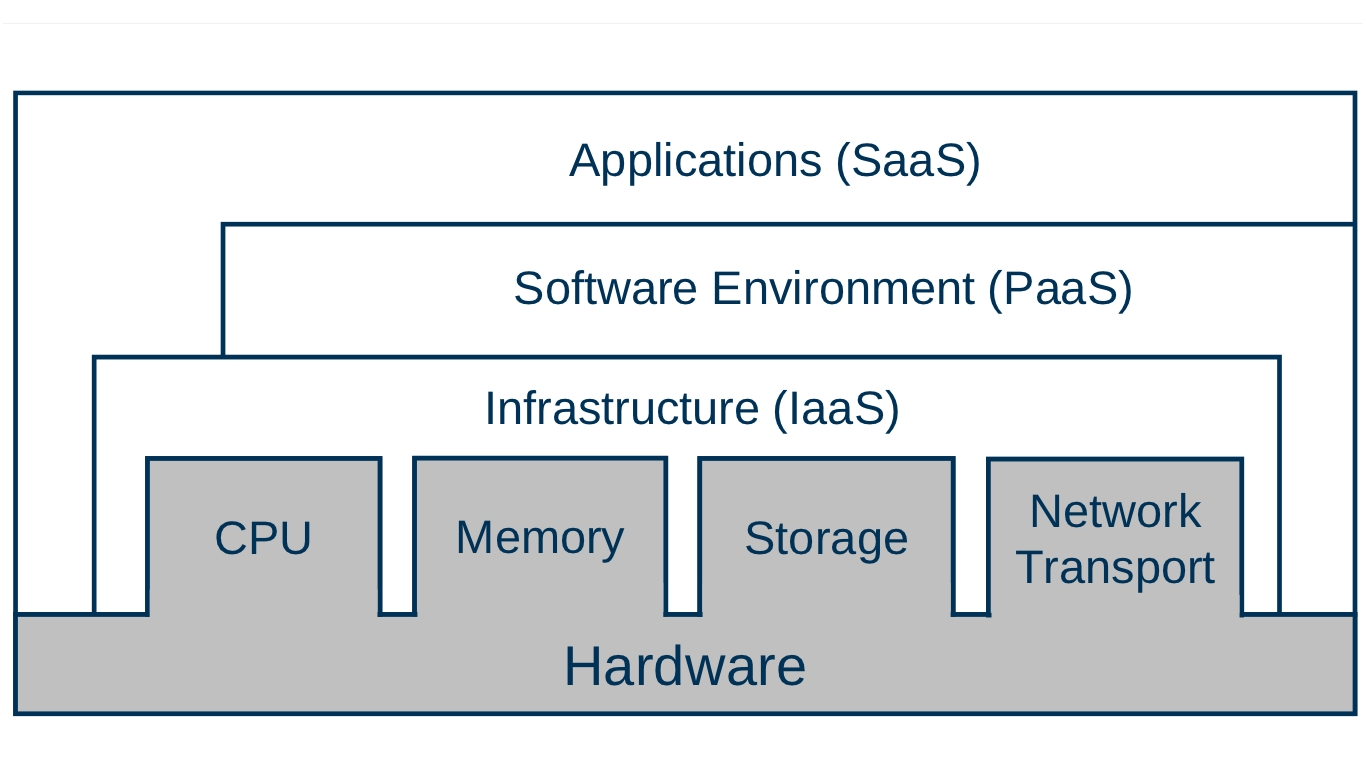
\includegraphics[scale=.2,keepaspectratio=true]{cclayers.jpg}
\end{center}
\end{frame}

\subsubsection{Saas}
\begin{frame}
\frametitle{Software as a Service}
\begin{itemize} [<+->]
 \item Directly consumed by the customers.
 \item No need to install and run the software.
 \item Simplify maintanence and support.
 \item \dots 
\end{itemize}
\end{frame}


\subsubsection{Paas} 
\begin{frame}
\frametitle{Platform as a Service}
\begin {itemize} [<+->]
 \item Consumed by developers or Tech Savvy individuals.
 \item Project environment ready for developers.
 \item Combinations of simplicity and cost efficiency.
 \item \dots
\end {itemize}
\end{frame}

\subsubsection{Iaas}
\begin{frame}
\frametitle{Infrastructure as a Service}
\begin{itemize} [<+->]
 \item Computer infrastructure - platform virtualisation environment
 \item Raw storage and Networking
 \item Servers,softwares,Data-center space or Network equipment
 \item Billing based on utility basis
\end{itemize}
\end{frame}

\begin{frame}
\begin{center}
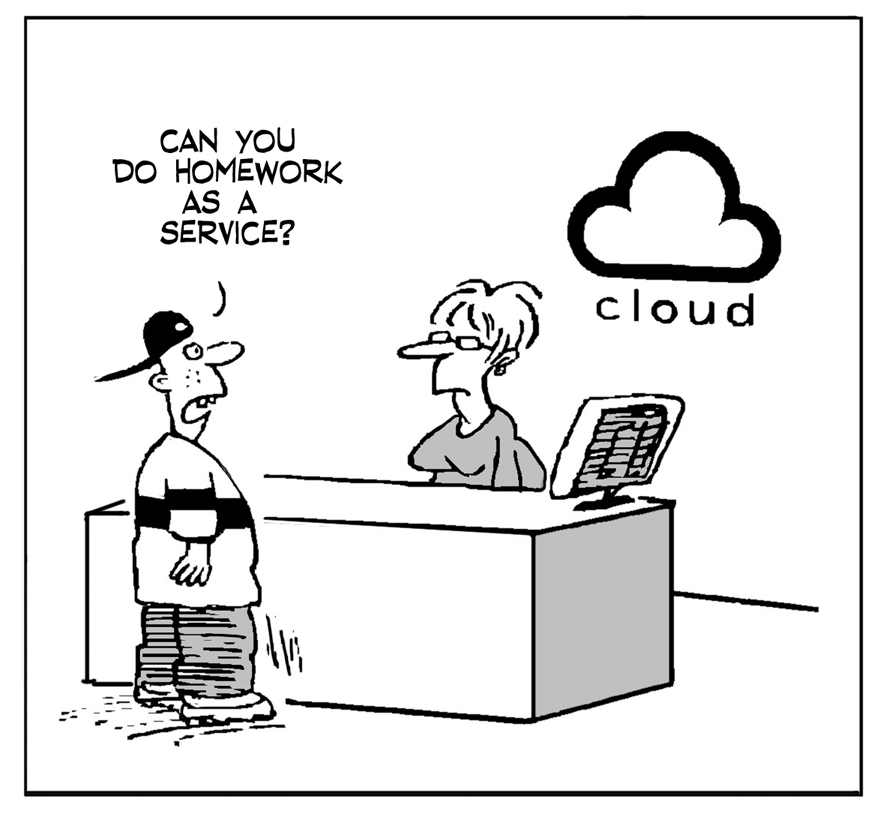
\includegraphics[scale=1.1,keepaspectratio=true]{2.jpg} 
\end{center}
\end{frame}

\section{Networking of Information}
\begin{frame}
\frametitle{Networking of Information}

  \begin{itemize} [<+->]
 
  \item No common persistent naming scheme for information.
    \begin{itemize} 
      \item Information named relative to the box they are located in, URL's resolve to IP-address.
	\begin{itemize}
	  \item Moving Information = Changing it's Name ("404" file not found errors).
	 \end{itemize}
    \end{itemize}

 \item Mobility and multihoming for hosts and networks is problematic due to semantic overload of IP-address.

  \end{itemize}
\end{frame}

\begin{frame}
\frametitle{Networking of Information (Contd..)}
  \begin{itemize} [<+->]
    \item No consistent representation of information (copy-independant).
      \begin{itemize} 
	\item No consistent ways to keep track of identical copies.
	\item Different encodings (eg: mp3,wav) worsen problem.
      \end{itemize}

    \item Security is host-centric.
      \begin{itemize}
	\item Mainly based on security channels (Encryption) and trusting servers (Authentication).
	\item Can't generally trust a copy received from an untrusted user.
      \end{itemize}

  \end{itemize}
\end{frame}

\begin{frame}
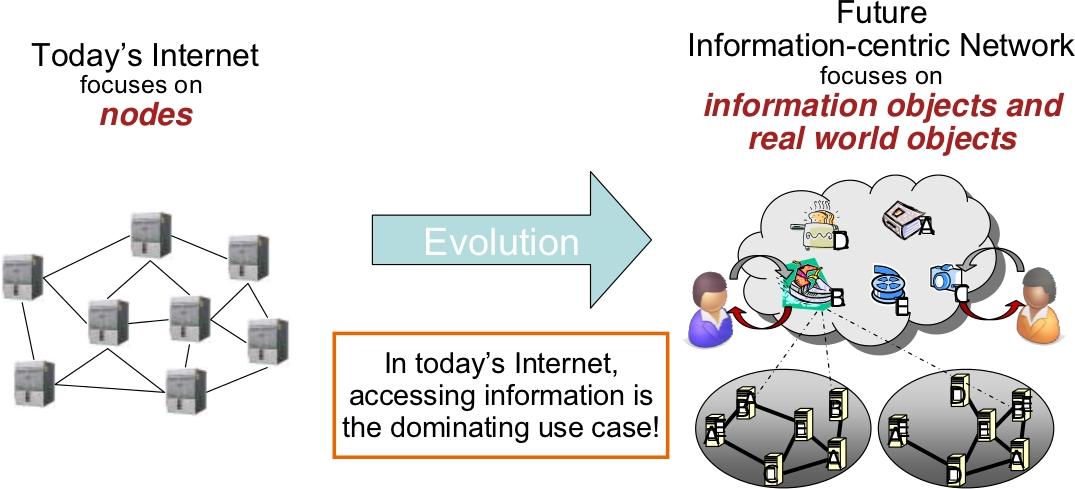
\includegraphics[scale=.3,keepaspectratio=true]{netinf1.jpg}
 \end{frame}


\subsection{NetInf Scenarios}

\begin{frame} 
  \frametitle{Content Distribution}
\pause 
    \begin{center}
         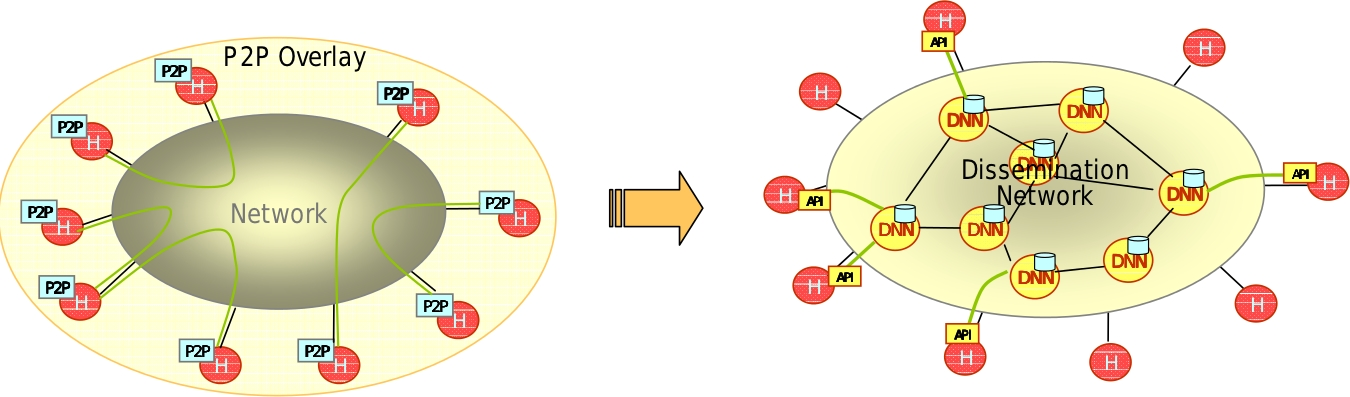
\includegraphics[keepaspectratio=true,scale=.22]{Netinf5.jpg}  
    \end{center}

 \begin{itemize} [<+->]
	\item VideoOnDemand, Live TV, Webpages.
	\item Caching can be built in from begining.
	\item Information can be retrieved from the closest available source.
	\item Common dissemination infrastructure for all applications, including network support.
     \end{itemize}
\end{frame}  

\begin{frame}
  \frametitle{Augmented Internet Real World Objects.}
    \begin{center}
      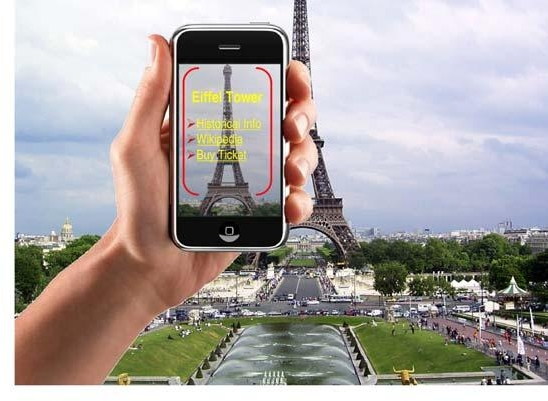
\includegraphics[keepaspectratio=true,scale=.26]{pic2.jpg}    
    \end{center}

\begin{itemize}
 \item Linking real world objects in the virtual information world.
 \item Clicking on and bookmarking real world objects.
\end{itemize}
\end{frame}


\begin{frame}
  \frametitle{Personal mobile scenario}
  \begin{center}
    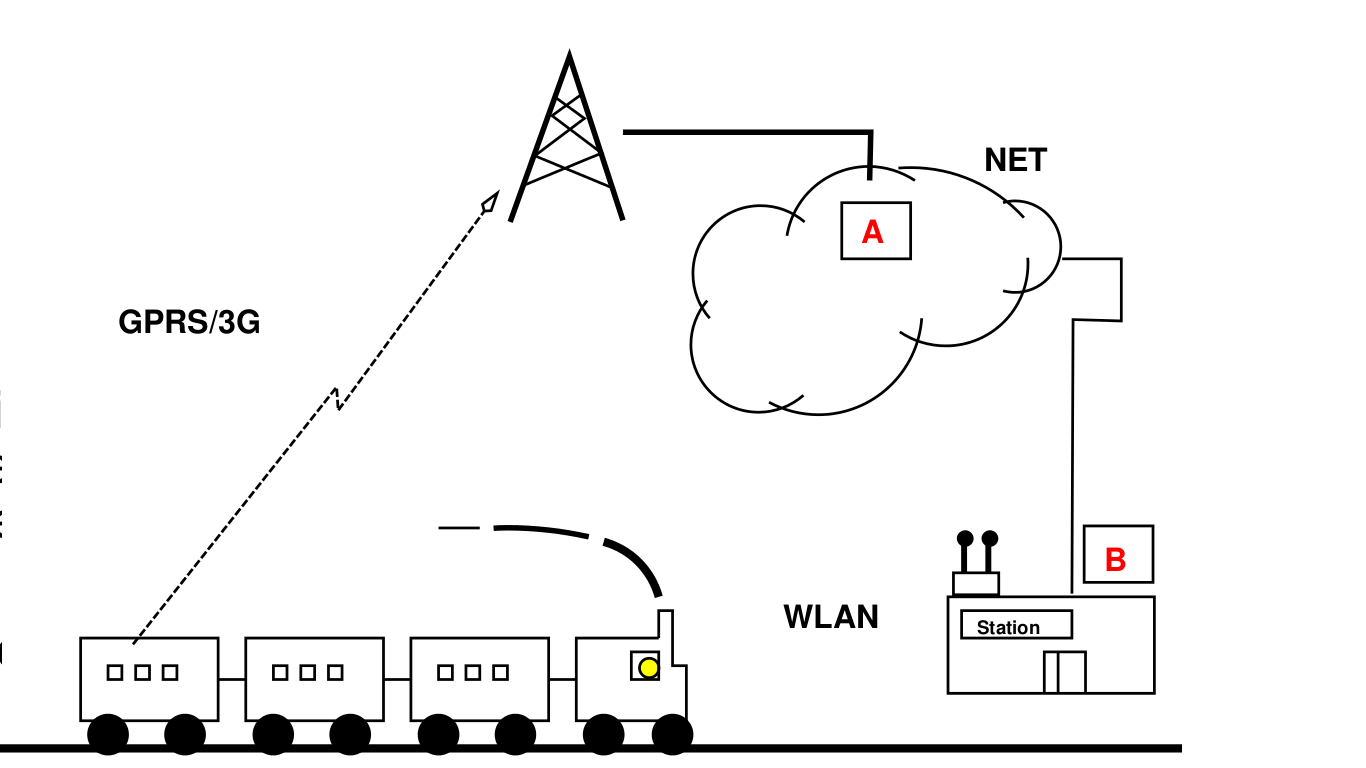
\includegraphics[keepaspectratio=true,scale=.13]{netinf7.png}
   
  \end{center}

\begin{itemize}
 \item Retrieving information when connectivity is intermittent, efficiently utilising high-bitrate access when available or using alternative sources.
 \item Information objects provides natural anchor points for multiaccess and multihoming.
\end{itemize}

\end{frame}



\begin{frame}
 \frametitle{API for locating any type of object}
\begin{center}
 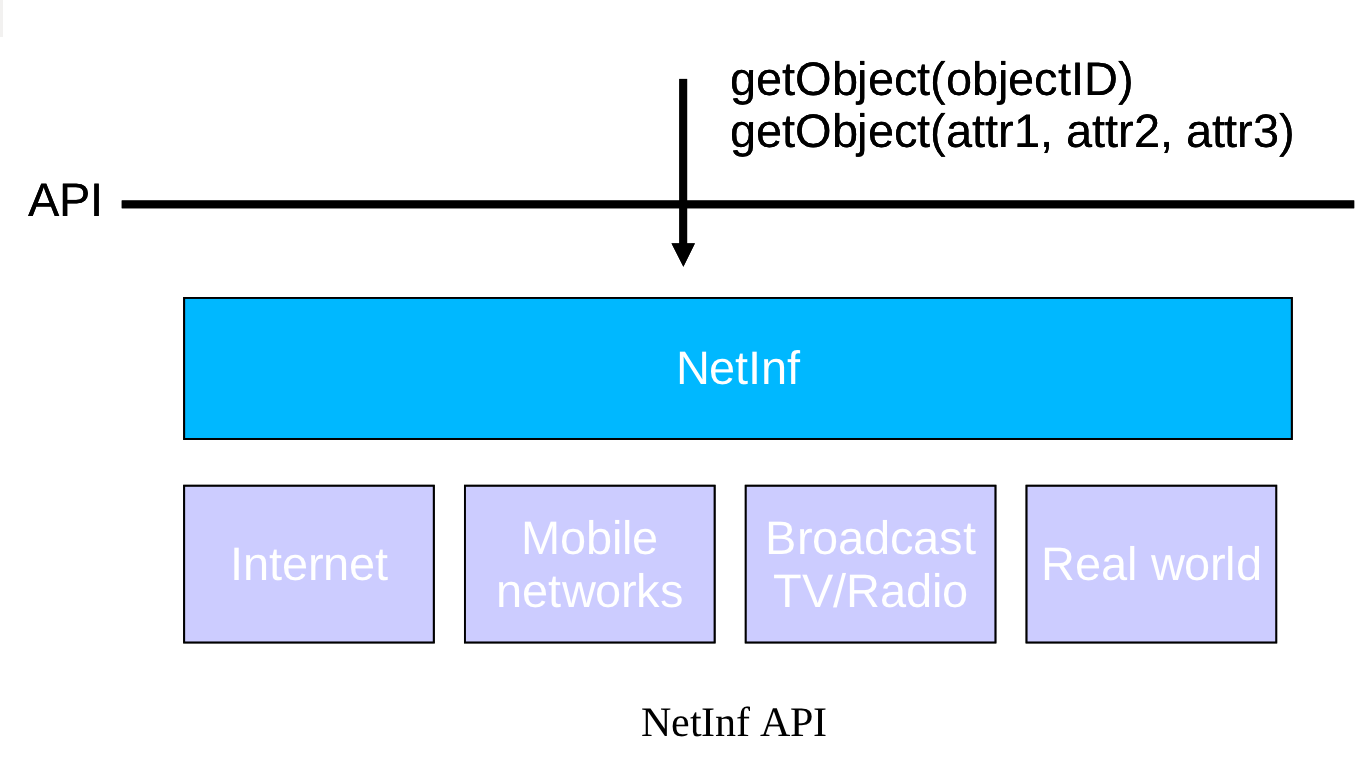
\includegraphics[scale=.2,keepaspectratio=true]{Netinf3.png}
\end{center}
\end{frame}

\begin{frame}
 \frametitle{Organize Information – Examples of Hierarchies}
  \begin{center}
    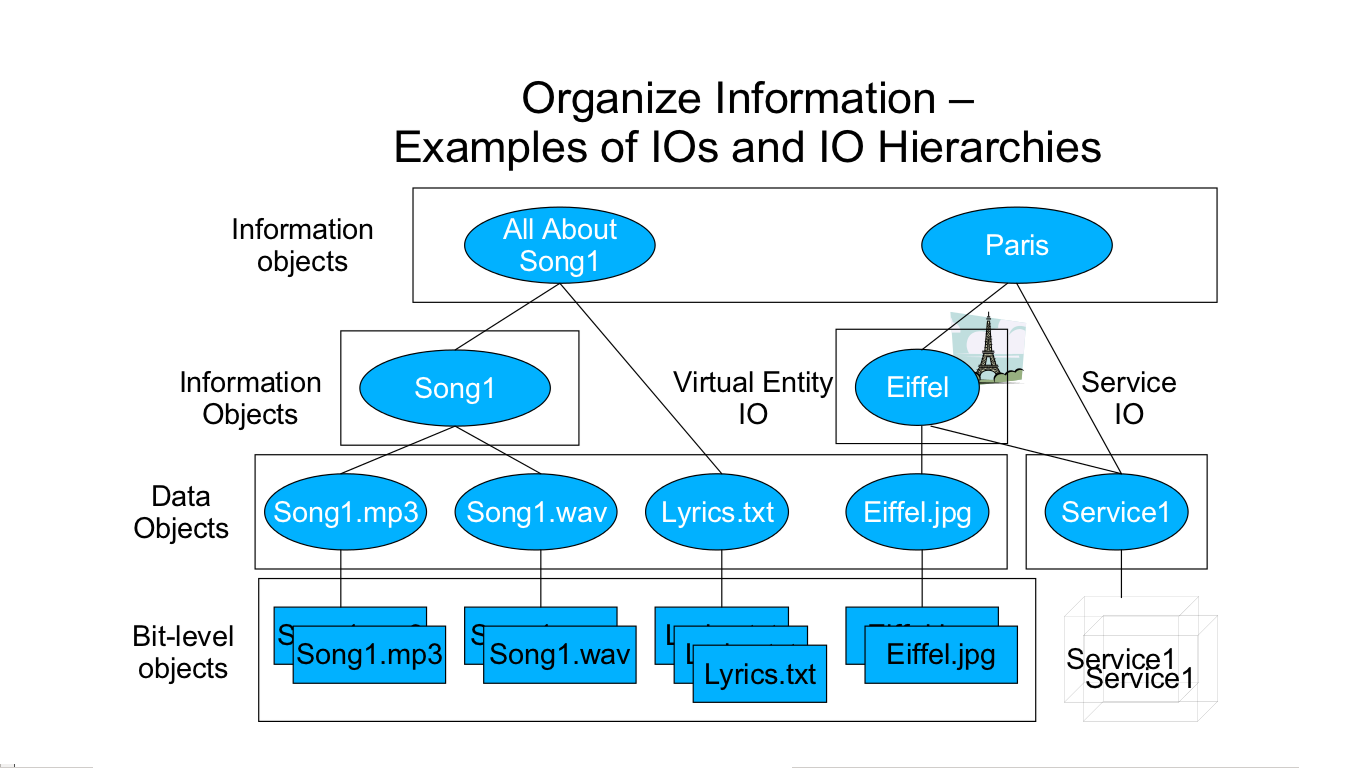
\includegraphics[keepaspectratio=true,scale=.22]{netinf2.png}
  \end{center}
\end{frame}

\subsection{NetInf Naming}
\begin{frame}
\frametitle{Naming Scheme}
\begin{center}
 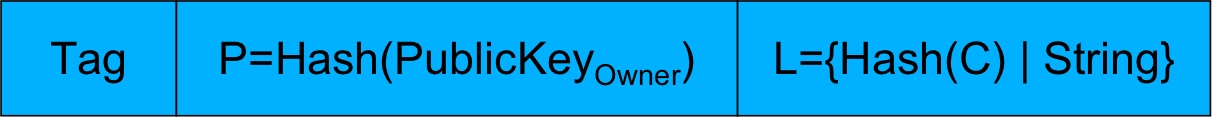
\includegraphics[keepaspectratio=true,scale=.24]{netinfnaming.jpg}
\end{center}
\begin{itemize}
 \item \textbf{Tag} : Defines the format
 \item \textbf{Principal (P)} : Object ‘publisher’ (optional)
 \item \textbf{Label (L)} : Identifying individual object published by Principal. 
\end{itemize}

\end{frame}


\begin{frame}
 \begin{center}
    \textbf{\emph{What does all that have to do with Cloud Computing ?}}
 \end{center}

\end{frame}

\section{NetInf meets Cloud Computing}
\begin{frame}
\frametitle{NetInf meets Cloud Computing}
\begin{itemize}
 \item Cloud-computing - a resource sharing paradigm
       \begin{itemize}
        \item E.g, computing power, storage,\dots
        \item Execute software on the web, pay-per-use (SaaS)
        \item Platforms for building and hosting services (PaaS)
        \item Deployment platforms (IaaS)
        \item \textbf{ Focus on the resource and what’s running on top}
       \end{itemize}
\item NetInf – a networking paradigm / technology
       \begin{itemize}
        \item Data-oriented networking paradigm
        \item \textbf{Focus on transporting and accessing data}
       \end{itemize}
\item Both very different in nature, but there are common aspects.
\end{itemize}

\end{frame}


\begin{frame}
\frametitle{NetInf meets Cloud Computing}
 \begin{center}
  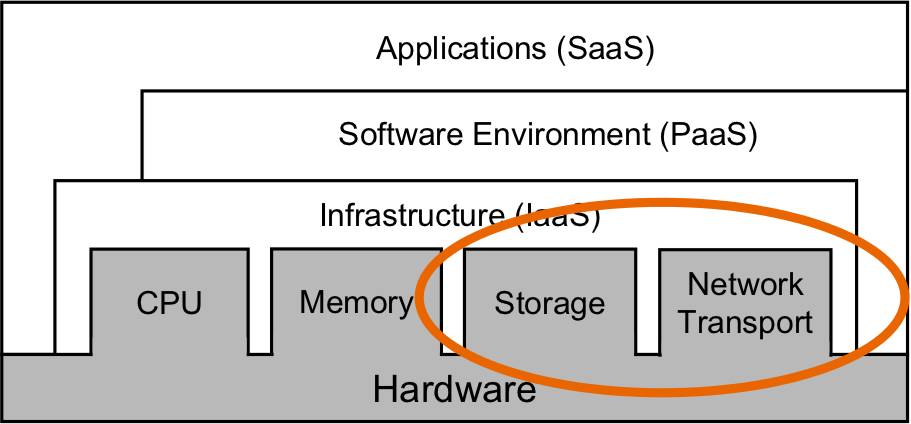
\includegraphics[keepaspectratio=true,scale=.25]{netinf8.png}
 \end{center}

\end{frame}


\section{Challenges in Cloud Computing}
\begin{frame}
\frametitle{Challenges in Cloud Computing}
\begin{itemize}
 \item Requires reasonably stable infrastructure
    \begin{itemize}
     \item E.g. not practical to deploy components in a moving network/home network scenarios.
    \end{itemize}
 \item  Inconsistent security mechanisms
    \begin{itemize}
     \item Per application.
     \item Host-centric (secure the channel, not the information).
    \end{itemize}
 \item Management can be fairly complex and expensive.
    \begin{itemize}
     \item Computing
     \item Storage
     \item Fecilities
    \end{itemize}

\end{itemize}
\end{frame}

\section{Summary and Conclusion}
 \begin{frame}
  \frametitle{Summary and Conclusion}
  \begin{itemize}
   \item The Cloud Architecture.
	  \begin{itemize}
	   \item Saas,Paas,Iaas,\dots
	  \end{itemize}

   \item Network architecture based on information-centric paradigm.
	  \begin{itemize}
	   \item Naming scheme for objects independent of nodes.
	   \item Scalable solution for node and network mobility and multihoming.
	   \item Enable efficient information dissemination
% 	   \item Secure information-centric architecture by embedding security into identifiers.
	   \item A common infrastructure and API for accessing all types of objects.
	   \item Scalable name to locator resolution for a large number of objects.
	   \item Designing NetInf to make it largely self-managing
	  \end{itemize}
\end{itemize}
\end{frame}

\begin{frame}
\frametitle{Summary and Conclusion (Contd..)}
\begin{itemize}
    \item Capable of improving the cloud computing infrastructure.
	  \begin{itemize}
	   \item Storage
	   \item Transport
	   \item Security
	   \item Directory
	   \item Integration with network virtualization
	  \end{itemize}

  \end{itemize}
\end{frame}


\begin{frame}
\frametitle{References}
\begin{enumerate}
 \item [[1]] What Networking of Information Can Do for Cloud Computing , Börje Ohlman, Anders Eriksson , René Rembarz. Ericsson Research , Ericsson. 
 \item [[2]] EU FP7 4WARD project, http://www.4ward-project.eu/
 \item [[3]] Rao Mikkilineni. Cloud Computing and the lLessons from the Past.2009.
 \item [[4]] www.wickipedia.org/cloud\_computing
 \item [[5]] www.wickipedia.org/dynamic\_dns
 \item [[6]] www.wickipedia.org/multihoming
 \item [[7]] www.wickipedia.org/virtualization
 \item [[8]] Cloud computing series in Techno-pulse.
\end{enumerate}
\end{frame}

\begin{frame}
 \begin{center}
  Thanks For your \textbf{Attention !!} \\[1 cm] 
  Time for Discussion.\\[2cm]
\emph{``A prudent question is one-half of wisdom.'' - Francis Bacon}
 \end{center}
\end{frame}


\end{document}

